%!TEX root = ../Thesis.tex
\section{Controller Tuning} % (fold)
\label{sec:controller_tuning}
The software modules node\_navigation, node\_aruco and node\_controller described in section~\ref{sec:implementation} are implemented and running in real time locally on the \gls{UAV}. Tests are conducted by manual takeoff and flight to a starting point at a distance from the landing pad. The \textit{do land} command is then triggered from the work station and the UAV, running the controller defined in chapter~\ref{cha:controller} performs autonomous landing. The parameters listed in \ref{tab:stateMachineParameters} are used in the implemented state machine.
\begin{table}[!htb]
  \centering
  \begin{tabular}{c|l|l}
    \toprule
    \textbf{Parameter}&\textbf{Description}&\textbf{Value}\\
    \hline
    $U_{c,max}$&Maximum UAV approach speed&$3m/s$\\
    $\Delta_1$&controller gain&$3.0$\\
    $\Delta_2$&controller gain after gain adjust&$2.0$\\
    $h$&Hover height&$15m$\\
    $r_h$&Radius of the hover sphere&$0.5m$\\
    $h_g$&Gain adjust altitude&$8.0m$\\
    $h_f$&Final stage altitude&$4.0m$\\
    $v_d$&Main decent velocity&$0.40m/s$\\
    $v_f$&Final stage decent velocity&$0.30m/s$\\
    $c_h$&Minimum covariance in hover&$100$\\
    $r_l$&Radius of the landing cylinder&$0.20m$\\
    $h_l$&Height of the landing cylinder&$0.50m$\\
    \bottomrule
  \end{tabular}
  \caption{Parameters used in the state machine}
  \label{tab:stateMachineParameters}
\end{table}

Figure~\ref{fig:controller_tuning} presents a plot of the relative position estimate between the \gls{UAV} and landing pad $\vect{p}^{n}_{l/u}$ calculated by the state estimator during the test. The states from the state machine are included in the figure as vertical lines marked with the state name.
\begin{figure}[h!]
	\centering
	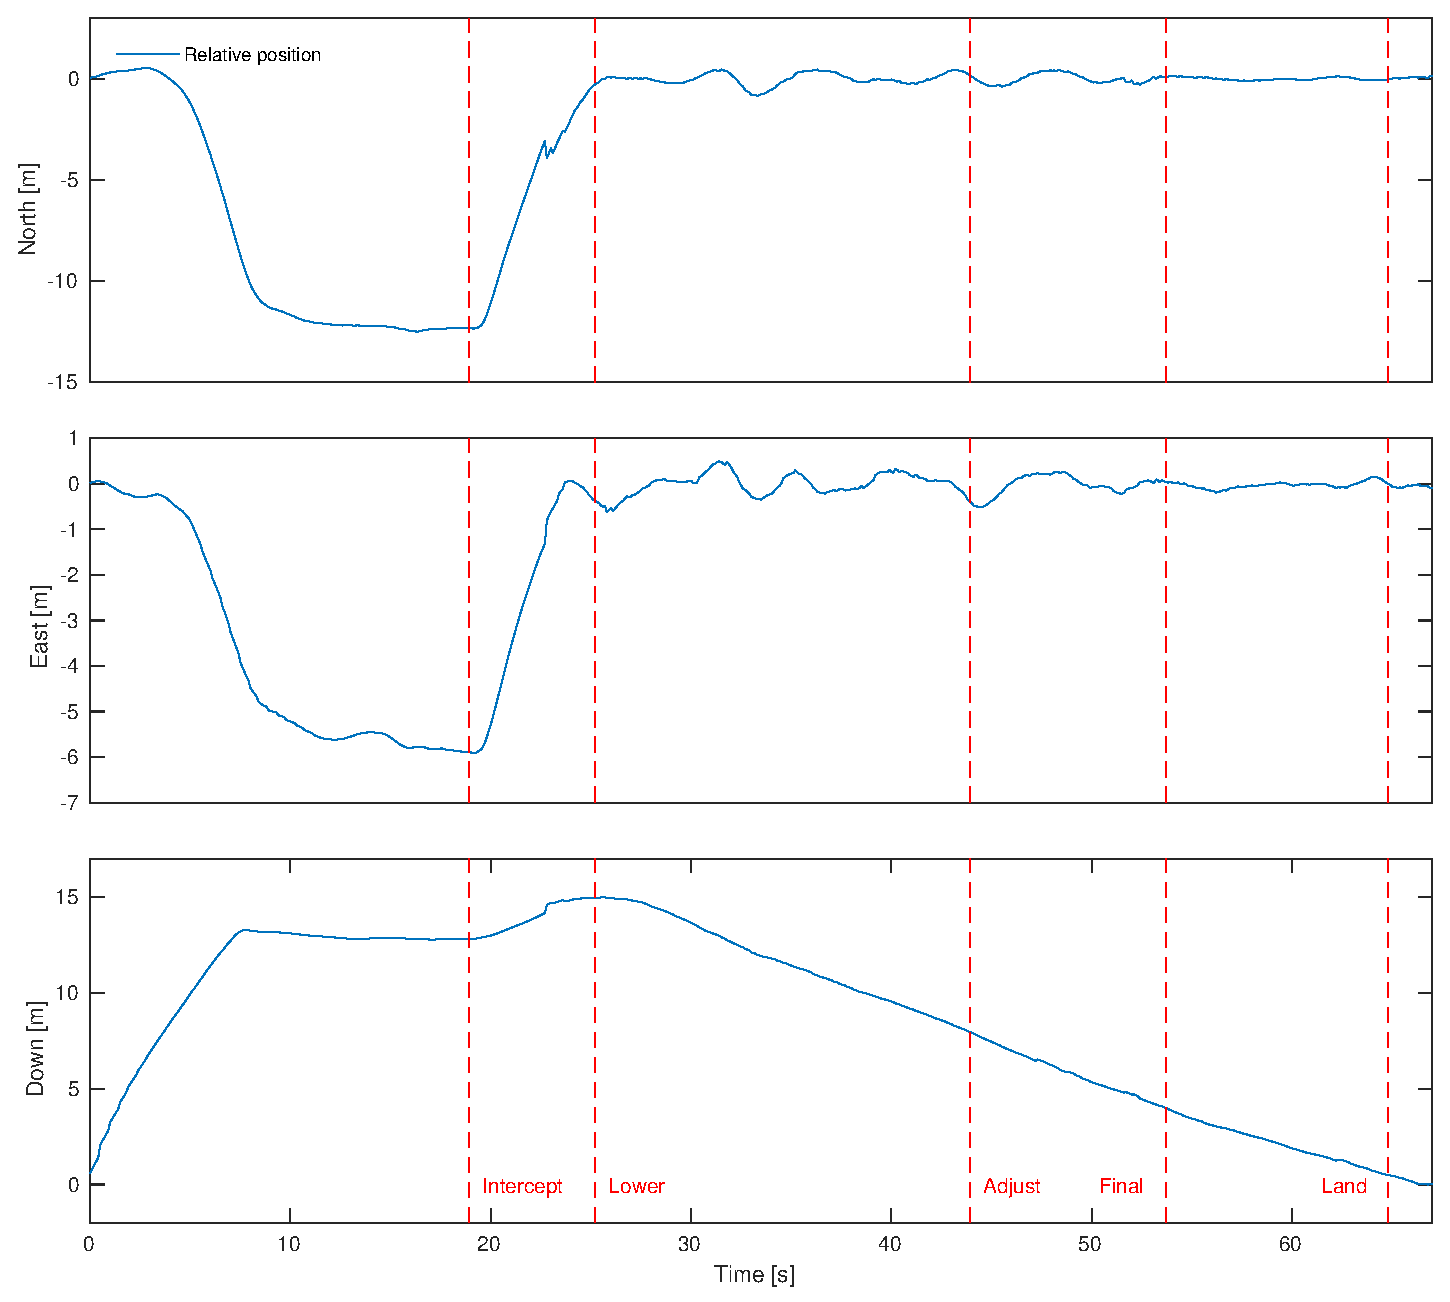
\includegraphics[width=.9\linewidth]{img/plot/static/controller.eps}
	\caption{Relative position $\vect{p}^{n}_{l/u}$ during autonomous landing}{Relative position $\vect{p}^{n}_{l/u}$ during autonomous landing. State machine states indicated by vertical lines}
	\label{fig:controller_tuning}
\end{figure}
Moreover, the \textit{Adjust} and \textit{Final} are abbreviations for \textit{Gain Adjust} and \textit{Final Stage}.

As indicated in figure~\ref{sec:controller_tuning}, the first 19 seconds of the flight is carried out manually. The state machine then enters the \textit{intercept} state and the UAV starts to fly towards the hovering point. From the \textit{intercept} phase in figure~\ref{fig:controller_tuning}, there is a "jump" in the position estimate. This is due to filter corrections in the appearance of AruCo measurements. The state machine goes straight from \textit{Intercept} state to \textit{Lower}, not including the \textit{Hover} state. This is a result of the high value set as parameter for the minimum covariance in hover $c_h$. The oscillations in the north and east position caused by the wind affecting the \gls{UAV}. During the Gain Adjust phase, the north and east position stabilizes, making the UAV stable trough the \textit{Final} state until it finally triggers the \textit{Land} command.


\subsection{Summary} % (fold)
\label{sub:controller_summary}
Several dozens of physical real-time test on a static landing pad have been conducted using the implemented software modules node\_navigation, node\_aruco and node\_controller. The autonomous system has given exceptional results, by performing precise and stable landings with high repeatability. A video of from one of the tests conducted can be seen at \url{https://youtu.be/H2HTWxUuOW8}
% subsection controller_summary (end)
% section controller_tuning (end)